% !TEX root = ../main.tex
% Бүлэг 3

\chapter{Арга зүй ба санал болгох архитектур}
\label{Chapter3}
\pagecolor{Beige}

%-------------------------------------------------------------------------------

\section{Судалгааны загвар}

Энэхүү судалгаа нь тоон судалгааны арга зүйд суурилсан туршилтын шинжтэй судалгаа болно. Судалгааны үндсэн зорилго нь ясны хугарлын рентген зурагт тулгуурлан хугарал илрүүлэх, хугарлын хэсгийг сегментлэх, хугарлын зэргийг үнэлэх болон эдгэрэлтийн төлөвийг таамаглах боломжийг гүн сургалтын аргаар судалж, загваруудын гүйцэтгэлийг тоон үзүүлэлтээр үнэлэхэд оршино.

Судалгааны явцад олон нийтэд нээлттэй рентген зургийн өгөгдлийн сангуудыг ашиглан гүн сургалтын загваруудыг сургаж, туршилтын үр дүнг холбогдох үнэлгээний хэмжүүрүүдээр тооцон харьцуулсан. Судалгааны ерөнхий үйл явц нь өгөгдөл цуглуулах, өгөгдөл боловсруулах, загвар хөгжүүлэх, загварыг турших, үр дүнг тайлбарлах гэсэн үндсэн үе шатуудаас бүрдэнэ.

Судалгааны ажлыг дараах дөрвөн үе шаттайгаар хэрэгжүүлэв.

\subsection*{Үе шат 1. Өгөгдөл бэлтгэх}

Энэ үе шатанд судалгаанд ашиглах өгөгдлийн эх сурвалжуудыг сонгон нэгтгэж, сургалтад ашиглахад шаардлагатай урьдчилсан боловсруулалтыг гүйцэтгэв. Үүнд рентген зургийн хэмжээг нэгэн ижил болгох, пикселийн утгыг нормчлох, өгөгдөл нэмэгдүүлэх, мөн өгөгдлийг сургалт, баталгаажуулалт болон тестийн багцад хуваах зэрэг ажиллагаа багтсан. Түүнчлэн өгөгдлийн сан бүрийг тухайн судалгааны даалгаврын онцлогт нийцүүлэн ангилан ашиглав.

\subsection*{Үе шат 2. Загвар хөгжүүлэлт ба сургалт}

Өгөгдөл бэлтгэсний дараа хугарал илрүүлэх, сегментлэх, хугарлын зэргийг үнэлэх болон эдгэрэлтийн төлөвийг таамаглах зориулалт бүхий гүн сургалтын загваруудыг боловсруулж сургав. Загваруудыг сургалтын өгөгдөл дээр сургаж, баталгаажуулалтын өгөгдлөөр гиперпараметр болон сургалтын тохиргоог оновчлов.

\subsection*{Үе шат 3. Үнэлгээ ба харьцуулалт}

Сургасан загваруудын гүйцэтгэлийг тухайн даалгаварт тохирох үнэлгээний хэмжүүрүүдээр үнэлэв. Ангиллын даалгаварт Accuracy, Precision, Recall, F1-score болон AUC зэрэг үзүүлэлтүүдийг ашигласан бол сегментчлэлийн даалгаварт Dice coefficient болон IoU үзүүлэлтүүдийг хэрэглэв. Үр дүнг суурь загварууд болон өмнөх судалгааны үр дүнтэй харьцуулан шинжилсэн.

\subsection*{Үе шат 4. Үр дүнгийн тайлбар ба дүн шинжилгээ}

Энэ үе шатанд загварын гаргасан шийдвэрийг тайлбарлах боломжийг судалж, рентген зургийн аль хэсэг нь шийдвэр гаргалтад хамгийн их нөлөөлж байгааг шинжилэв. Мөн туршилтын үр дүнг өмнөх судалгаануудтай харьцуулан дүгнэж, санал болгож буй аргын давуу тал, хязгаарлалт болон цаашдын судалгааны боломжит чиглэлүүдийг тодорхойлов.

%-------------------------------------------------------------------------------

\section{Хугарал илрүүлэх, сегментлэх ба хугарлын зэрэг үнэлэх архитектур}
\label{sec:arch_v1}

Энэхүү судалгаанд рентген зурагт суурилан хугарал байгаа эсэхийг тодорхойлох, хугарлын хэсгийг сегментлэх, хугарлын зэргийг үнэлэх, улмаар эдгэрэлтийн хугацааг таамаглах дараалсан зорилт бүхий архитектурыг боловсруулав. Эдгээр даалгавар нь хоорондоо уялдаатай боловч суралцах шинж чанар, өгөгдлийн тэмдэглэгээ, үнэлгээний хэмжүүрийн хувьд ялгаатай. Иймээс архитектурыг боловсруулахдаа нэг талаас даалгавруудын хоорондын мэдээллийн хамаарлыг ашиглах, нөгөө талаас нэг даалгаврын алдаа дараагийн даалгаварт хэт хүчтэй нөлөөлөхөөс сэргийлэх зарчмыг баримталсан.

Судалгааны явцад архитектурын гурван өөр хувилбарыг дараалан туршсан: (а) нэг хуваалцсан кодлогчтой нэгдсэн олон даалгаварт (multi-task) загвар, (б) даалгавар тус бүрийг тусдаа загвараар дараалан сургах арга, болон (в) эцсийн модульчлагдсан каскад pipeline. Эдгээр гурван хувилбарын бүтцийн ялгааг Зураг~\ref{fig:three_arch}-д харьцуулан үзүүлэв.

\begin{figure}[!htbp]
\centering
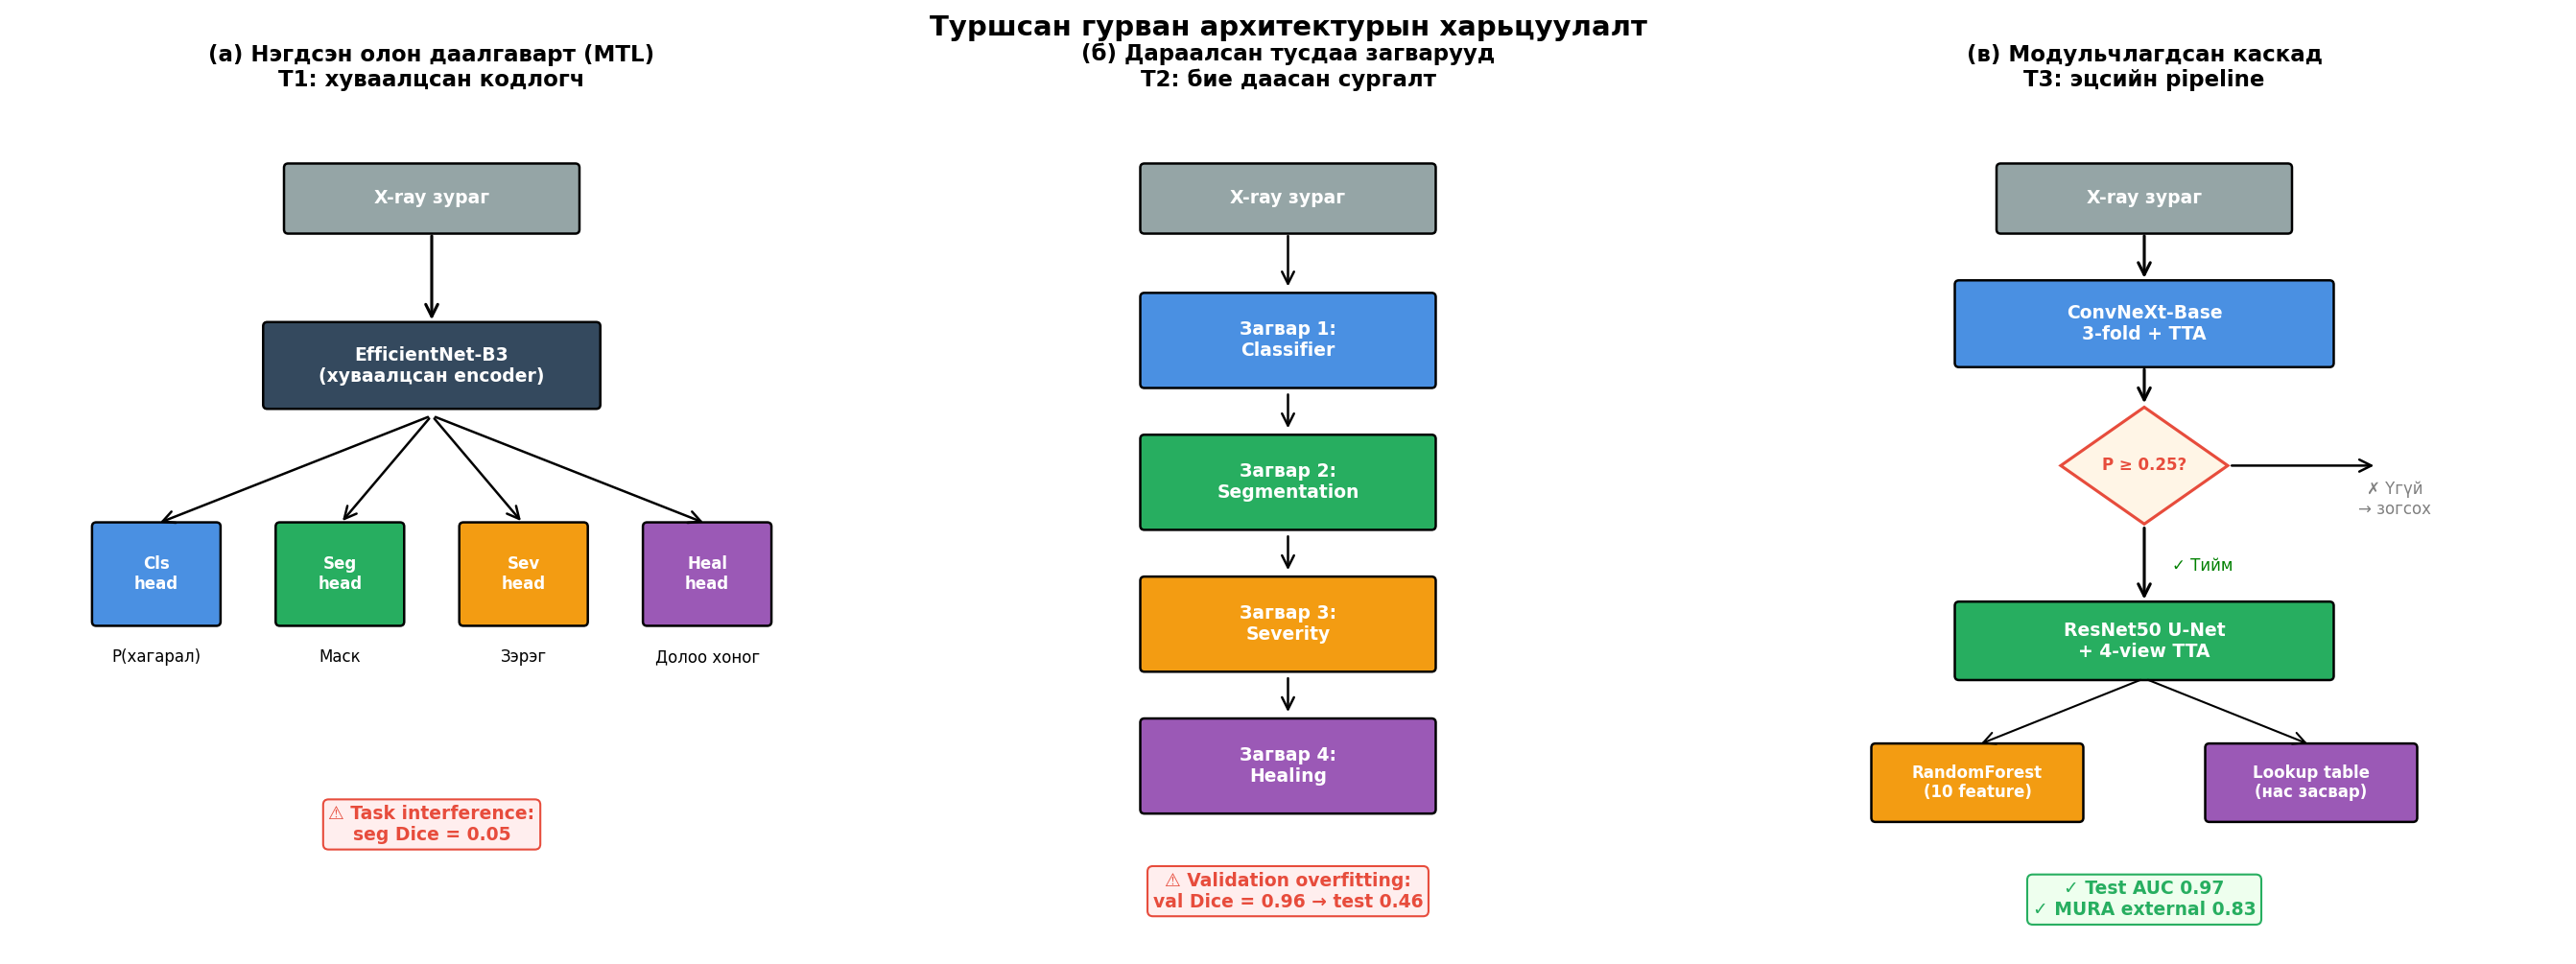
\includegraphics[width=\textwidth]{Figures/Figure_3_1.png}
\figcaption{Туршсан гурван архитектурын харьцуулалт}{Судалгааны явцад туршсан гурван архитектур: (а) нэгдсэн олон даалгаварт (MTL) хуваалцсан кодлогч, (б) дараалсан/тусдаа сургасан загварууд, (в) эцсийн модульчлагдсан каскад pipeline}
\label{fig:three_arch}
\end{figure}

Судалгааны эхний хувилбарт нэг хуваалцсан кодлогч дээр суурилсан олон даалгаварт загвар туршсан. Энэ хувилбарын зорилго нь нэг рентген зургаас нийтлэг дүрслэлийн шинж чанарыг ялган авч, түүнийг ангилал, сегментчлэл, хугарлын зэрэг болон эдгэрэлтийн таамаглалын модулиудад зэрэг ашиглах явдал байв. Харин туршилтын явцад сегментчлэлийн даалгавар бусад даалгавартай хамт сургах үед тогтворгүй болох хандлага илэрсэн тул эцсийн шийдэлд даалгавар тус бүрийг бие даасан модулиар шийдвэрлэх каскад pipeline-ийг сонгосон. Энэ шийдэл нь загвар бүрийг өөрийн өгөгдөл, алдагдлын функц, сургалтын тохиргоонд нь нийцүүлэн оновчлох боломж олгосон.

\subsection{Туршилт 1: хуваалцсан кодлогчтой олон даалгаварт архитектур}

Анхны архитектурын үндсэн кодлогчоор ImageNet дээр урьдчилан сургагдсан EfficientNet-B3 загварыг сонгосон. EfficientNet-B3 нь compound scaling зарчмаар сүлжээний гүн, өргөн болон оролтын нарийвчлалыг тэнцвэртэй өсгөдөг тул харьцангуй цөөн параметртэй боловч дүрсний төлөөлөл гаргах чадвар сайтай архитектур юм~\cite{ref38}. Кодлогчийн сүүлийн feature map-аас Global Average Pooling ашиглан 384 хэмжээст төлөөлөл үүсгэж, үүнийг дараах дөрвөн модулийн оролт болгон ашигласан.

Нэгдүгээрт, ангиллын модуль нь рентген зурагт хугарал байгаа эсэхийг хоёртын ангиллын хэлбэрээр тодорхойлно. Энэ модуль нь кодлогчоос авсан төлөөллийг бүрэн холболтын давхаргуудаар боловсруулж, хугаралтай болон хугаралгүй гэсэн хоёр гаралт үүсгэнэ. Хоёрдугаарт, сегментчлэлийн модуль нь хугарлын хэсгийг пикселийн түвшинд ялгах зорилготой бөгөөд U-Net хэлбэрийн decoder салбарыг ашигласан. Ингэснээр кодлогчийн гаргасан өндөр түвшний шинжүүдийг decoder хэсгээр орон зайн маск болгон сэргээж, ангилал ба сегментчлэлийг нэг архитектурт зэрэг сургах боломж бүрдсэн.

Гуравдугаарт, хугарлын зэргийн модуль нь хугарлын маск болон дүрсний төлөөллийг хамтад нь ашиглан 0--3 зэрэглэлийн үнэлгээ гаргана. FracAtlas өгөгдлийн сангийн хугарлын зэргийн анхны шошго бүрэн биш байсан тул маскийн талбайн харьцаанд үндэслэн прокси зэрэглэл үүсгэж, зэрэглэлийн дараалсан шинжийг хадгалах үүднээс ordinal regression~\cite{ref35} ашигласан. Дөрөвдүгээрт, эдгэрэлтийн таамаглалын модуль нь дүрсний төлөөлөл, хугарлын зэргийн мэдээлэл болон нас, хүйс, анатомийн байршил зэрэг клиникийн мета-өгөгдлийг нэгтгэн эдгэрэлтийн хугацааг долоо хоногоор таамаглах регрессийн даалгавар болгон загварчилсан~\cite{ref43}.

Энэхүү олон даалгаварт хувилбар нь даалгавруудын хооронд мэдлэг хуваалцах боломжтой боловч туршилтын үр дүнгээс харахад сегментчлэлийн даалгаварт сөргөөр нөлөөлөх буюу task interference илэрсэн. Ялангуяа жижиг талбай эзэлдэг хугарлын маск нь ангилал болон регрессийн алдагдлын нөлөөнд дарагдаж, загвар хоосон маск гаргах хандлагатай болсон. Иймээс олон даалгаварт хандлага нь судалгааны чухал эхний алхам болсон боловч эцсийн pipeline-д шууд ашиглахад хангалттай тогтвортой биш гэж үзсэн.

\subsection{Туршилт 2: даалгавар тус бүрийг тусдаа сургах дараалсан архитектур}

Олон даалгаварт хувилбарын task interference-ийг бууруулах зорилгоор хоёр дахь хувилбарт даалгавар бүрийг нэг архитектурт нэгтгэхгүйгээр, тусдаа загваруудаар дараалан сургах аргыг туршсан. Энэ хувилбарт ангиллын загварыг MURA өгөгдөл дээр, сегментчлэл болон хугарлын зэргийн загварыг FracAtlas дээр, эдгэрэлтийн загварыг GRAZPEDWRI-DX-ийн мета-өгөгдөлд тулгуурлан тус тусад нь сургав. Модуль бүр өөрийн алдагдлын функц, оролтын хэмжээ болон сургалтын тохиргоотой байсан тул нэгдсэн загвартай харьцуулахад сегментчлэлийн сургалт мэдэгдэхүйц тогтворжсон.

Гэвч энэхүү хувилбарт сегментчлэлийн загвар баталгаажуулалтын олонлог дээр маш өндөр Dice (\(\approx 0.96\)) үзүүлсэн ч энэ нь баталгаажуулалтын өгөгдөлд хэт тохирох (overfitting) шинжтэй байсан тул бие даасан тест олонлог дээр ерөнхийлөх чадвар нь хангалтгүй байв. Иймээс дараалсан сургалт нь зөв чиглэлийн алхам боловч сегментчлэлийн жинхэнэ тогтворжилт болон ерөнхийлөх чадварыг бүрэн хангаагүй гэж дүгнэв. Энэ ажиглалт нь сургалтын стратеги (хоёр үе шаттай урьдчилсан сургалт, чанарын шүүлтүүр, TTA) болон илүү хүчтэй кодлогч шаардлагатайг харуулсан бөгөөд эцсийн модульчлагдсан хувилбарыг боловсруулах үндэслэл болсон.

\subsection{Туршилт 3: ConvNeXt ба ResNet50 U-Net-д суурилсан модульчлагдсан архитектур}

Эцсийн архитектур нь даалгавар тус бүрийг тусдаа загвараар шийдвэрлэх каскад бүтэцтэй. Энэ бүтэц нь эмнэлзүйн ажлын дараалалтай нийцнэ: эхлээд хугарал байгаа эсэхийг шалгаж, хугарал илэрсэн тохиолдолд байршлыг нь тодорхойлж, дараа нь хугарлын зэргийг үнэлэн эдгэрэлтийн хугацааг тооцно. Ийнхүү ангиллын модуль нь pipeline-ийн эхний шүүлтүүрийн үүрэгтэй, сегментчлэлийн модуль нь тайлбарлагдах байршлын мэдээлэл өгдөг, хугарлын зэргийн модуль нь маскаас гарсан морфологийн шинжүүдийг ашигладаг, эдгэрэлтийн модуль нь дүрс болон клиникийн мэдээллийг нэгтгэн регрессийн таамаглал гаргадаг.

Ангиллын модульд ImageNet-22K дээр урьдчилан сургагдсан ConvNeXt архитектурыг ашигласан. ConvNeXt нь CNN-ийн орон зайн inductive bias-ийг хадгалсан боловч орчин үеийн vision transformer загваруудын сургалтын зарим зарчмыг тусгасан тул эмнэлгийн дүрсний нарийн ялгааг танихад тохиромжтой гэж үзсэн. Ангиллын толгой нь бинар сигмоид гаралттай бөгөөд ангийн тэнцвэргүй байдлыг бууруулахын тулд Focal BCE алдагдал~\cite{ref44}, жинлэсэн sampling болон өгөгдөл нэмэгдүүлэх аргуудыг хэрэглэсэн.

ConvNeXt-ийг сонгосон үндсэн шалтгаан нь рентген зураг дээрх хугарлын шинж нь ихэвчлэн жижиг, локал, контраст багатай бүтэц хэлбэрээр илэрдэгтэй холбоотой. Уламжлалт CNN загварууд ийм орон зайн шинжийг сайн хадгалдаг боловч гүнзгий шатанд мэдээлэл бүдгэрэх, жижиг ан цавын ялгаа дарагдах эрсдэлтэй. ConvNeXt-ийн том kernel бүхий depthwise convolution, шаталсан feature hierarchy, LayerNorm болон GELU-д суурилсан блокийн бүтэц нь ийм нарийн дүрслэлийн ялгааг илүү тогтвортой ялгах боломжтой гэж үзсэн.

Мөн ImageNet-22K дээр урьдчилан сургасан ConvNeXt-Base хувилбар нь ImageNet-1K дээр сургасан жижиг загваруудаас илүү өргөн дүрслэлийн төлөөлөл сурсан байдаг. Эмнэлгийн рентген зураг нь судалгааны өгөгдлийн хэмжээгээр хязгаарлагдмал тул том хэмжээний ерөнхий дүрсний өгөгдөл дээр сурсан backbone ашиглах нь overfitting-ийг бууруулах, олон эх сурвалжийн зураг дээр ерөнхийлөх чадварыг нэмэгдүүлэх давуу талтай. Туршилтын харьцуулалтаар ConvNeXt-Base нь ResNet-50, EfficientNet-B3 болон ConvNeXt-Small загваруудаас өндөр AUC, F1 үзүүлсэн тул эцсийн ангиллын модуль болгон сонгосон.

Сегментчлэлийн модульд ResNet50~\cite{he2016resnet} кодлогчтой U-Net~\cite{ronneberger2015unet} архитектурыг ашигласан. Анхны $224\times224$ хэмжээ нь нарийн хугарлын шугамыг хангалттай хадгалж чадахгүй байсан тул сегментчлэлийн оролтыг $512\times512$ болгож нэмэгдүүлсэн. U-Net-ийн skip connection бүтэц нь доод түвшний ирмэг, хэлбэрийн мэдээллийг decoder хэсэгт шууд дамжуулдаг тул жижиг, нарийн хугарлын бүсийг сэргээхэд илүү тохиромжтой. Сургалтад FracAtlas-ийн гараар тэмдэглэсэн маскуудаас гадна SAM-аар үүсгэсэн псевдо маскуудыг чанарын шүүлтүүрээр дамжуулан ашигласан.

Хугарлын зэргийн үнэлгээнд зөвхөн хар хайрцаг хэлбэрийн ангилагч ашиглахын оронд сегментчлэлийн маскаас талбай, хэлбэр, чиглэл, хэсгийн тоо зэрэг морфологийн шинжүүдийг тооцох хандлага сонгосон. Энэ нь хугарлын зэрэглэлийг тайлбарлах боломжийг нэмэгдүүлж, эмч тухайн үнэлгээ ямар дүрсний шинжид үндэслэснийг шалгах нөхцөл бүрдүүлнэ. Гэхдээ хугарлын зэргийн шошго нь эмчийн бүрэн клиникийн үнэлгээ биш, морфологийн шинжид суурилсан прокси үнэлгээ тул энэ модулийг клиникийн баталгаажсан зэрэглэл тогтоогч бус, proof-of-concept түвшний модуль гэж авч үзсэн.

Эдгэрэлтийн модуль нь хугарлын зэрэг, анатомийн байршил, нас, хүйс зэрэг шинжүүдийг ашиглан эдгэрэлтийн хугацааг долоо хоногоор таамаглах регрессийн загвар хэлбэрээр боловсруулагдсан. Гэхдээ энэ хэсэгт бодит урт хугацааны клиникийн follow-up өгөгдөл дутагдалтай тул синтетик өгөгдөл ашигласан нь судалгааны нэг үндсэн хязгаарлалт болно. Иймээс эдгэрэлтийн модулийн үр дүнг мөн proof-of-concept буюу цаашид бодит клиникийн өгөгдлөөр баталгаажуулах шаардлагатай боломжийн баталгаа гэж тайлбарлав.

\subsection{Эцсийн pipeline-ийн оролт, завсрын гаралт ба шийдвэрийн урсгал}

Санал болгож буй pipeline-ийн ажиллагааг дараах дарааллаар нэгтгэн тодорхойлж болно.

\begin{enumerate}[nosep]
    \item Оролтын рентген зургийг стандарт хэмжээнд хөрвүүлж, нормчлол болон шаардлагатай нэмэлт боловсруулалтыг гүйцэтгэнэ.
    \item Ангиллын загвар зурагт хугарал байх магадлалыг тооцно. Хэрэв магадлал тогтоосон босгоос бага бол зураг хугаралгүй гэж тэмдэглэгдэж, дараагийн модулиуд ажиллахгүй.
    \item Хугарал илэрсэн зурагт сегментчлэлийн загвар ажиллаж, хугарлын бүсийн хоёртын маскийг үүсгэнэ.
    \item Маскаас морфологийн шинжүүдийг тооцож, хугарлын зэргийг 0--3 шатлалаар үнэлнэ.
    \item Дүрсний болон клиникийн шинжүүдийг нэгтгэн эдгэрэлтийн хугацааны таамаглалыг гаргана.
\end{enumerate}

Энэхүү бүтэц нь нэг загвараар бүх даалгаврыг зэрэг шийдвэрлэхээс илүү уян хатан бөгөөд аль нэг модульд сайжруулалт хийхэд бусад хэсгийг бүхэлд нь дахин сургах шаардлагыг бууруулна. Мөн ангиллын итгэлийн оноо, сегментчлэлийн маск, морфологийн шинжүүд зэрэг завсрын гаралтууд нь загварын шийдвэрийг тайлбарлах боломжийг нэмэгдүүлдэг. Иймээс санал болгож буй архитектурыг бие даасан оношилгооны систем бус, харин эмчийн шийдвэрийг дэмжих судалгааны түвшний pipeline гэж үзнэ.

%-------------------------------------------------------------------------------

\section{Өгөгдөл цуглуулах арга}

Судалгаанд ашиглах өгөгдлийг сонгохдоо хоёр үндсэн шалгуурыг баримталсан. Нэгдүгээрт, өгөгдлийн сан нь рентген зурагт суурилсан ясны хугарлын судалгаанд ашиглах боломжтой, нийтэд нээлттэй, судалгааны зориулалтаар ашиглах нөхцөл нь тодорхой байх шаардлагатай. Хоёрдугаарт, өгөгдөл нь энэхүү ажлын дөрвөн үндсэн даалгаврын аль нэгийг дэмжихүйц шошго, тэмдэглэгээ эсвэл мета-өгөгдөл агуулсан байх ёстой. Иймээс нэг өгөгдлийн сангаар бүх даалгаврыг шийдвэрлэх боломжгүй тул хэд хэдэн эх сурвалжийг зорилтот даалгаварт нь тохируулан нэгтгэн ашиглав.

Ангиллын даалгаврын өгөгдлийг туршилтын үе шат бүрийн зорилгод нийцүүлэн сонгосон. Эхний хоёр туршилтад MURA өгөгдлийн санг хэвийн болон гажигтай рентген зургийг ялгах суурь сургалтад ашигласан~\cite{ref39}. Харин эцсийн буюу гурав дахь туршилтын ангиллын модульд GRAZPEDWRI-DX, FracAtlas-COCO, YOLOBoneFracture болон BoneFractureCVProject өгөгдлийн сангуудыг нэгтгэн ашигласан~\cite{ref40,ref41}. Эдгээр эх сурвалжийг нэгтгэснээр хугаралтай болон хугаралгүй жишээний төрөлжилтийг нэмэгдүүлж, ангиллын загвар нэг өгөгдлийн сангийн дүрсний хэв шинжид хэт тохирох эрсдэлийг бууруулахыг зорьсон.

Сегментчлэлийн даалгаварт FracAtlas-ийн масктай зургуудыг үндсэн эх сурвалж болгон авсан. Гэвч гараар тэмдэглэсэн масктай зураг цөөн тул YOLOBoneFracture болон BoneFractureCVProject өгөгдлийн сангийн хайрцаг тэмдэглэгээг ашиглан SAM-д суурилсан псевдо маск үүсгэж, сегментчлэлийн сургалтын өгөгдлийг өргөтгөсөн. Энэ шийдэл нь хугарлын бүсийг пикселийн түвшинд суралцахад шаардлагатай жишээний тоог нэмэгдүүлэх зорилготой бөгөөд псевдо шошгоны чанарыг тусгай шүүлтүүрээр шалгасан.

Хугарлын зэргийн үнэлгээнд FracAtlas-ийн сегментчлэлийн маск болон түүнээс тооцоолсон морфологийн шинжүүдийг ашигласан. Анхны өгөгдлийн сан дахь хугарлын зэргийн шошго бүрэн биш тул хугарлын маскийн талбай, хэлбэр, чиглэл зэрэг дүрсний шинжид тулгуурлан зэрэглэлийн прокси мэдээлэл үүсгэсэн. Энэ нь эмчийн клиникийн үнэлгээг бүрэн орлохгүй боловч хугарлын дүрслэлийн хэмжигдэхүйц шинжүүд хугарлын зэрэгтэй хэрхэн уялдахыг турших боломж олгосон.

Эдгэрэлтийн таамаглалын хувьд ашигласан нээлттэй рентген зургийн сангуудад бодит эдгэрэлтийн хугацааны урт хугацааны шошго байхгүй байсан. Иймээс GRAZPEDWRI-DX-ийн нас, хүйс зэрэг мета-өгөгдлийг ашиглахын зэрэгцээ эмнэлзүйн лавлагаанд суурилсан синтетик клиникийн өгөгдөл үүсгэн туршилтын түвшинд хэрэглэв. Синтетик өгөгдөл нь бодит өвчтөний мэдээлэл агуулаагүй тул нууцлалын эрсдэл багатай боловч клиникийн бодит өгөгдлийг бүрэн төлөөлөхгүй. Иймээс эдгэрэлтийн модулийн үр дүнг судалгааны туршилтын хүрээнд тайлбарлав.

Өгөгдлийн сан бүрийн лиценз, ёс зүйн нөхцөл, урьдчилсан боловсруулалт, хуваалт болон чанарын шалгалтыг \ref{Chapter4}~бүлэгт дэлгэрэнгүй авч үзсэн. Энэ хэсэгт зөвхөн өгөгдлийн эх сурвалжуудыг ямар үндэслэлээр сонгож, судалгааны даалгавруудад хэрхэн хуваарилсныг нэгтгэн тодорхойлов.

%-------------------------------------------------------------------------------

\section{AI хэрэгслийн ашиглалт ба ил тод байдал}

Судалгааны ажлын явцад хиймэл оюунд суурилсан туслах хэрэгслийг зөвхөн хязгаарлагдмал, туслах зориулалтаар — бичвэрийн найруулга, үг үсэг, хэл зүйн алдаа шалгах, \LaTeX{} форматлалыг тодруулах болон кодын алдаа засахад зөвлөмж авахад ашигласан. Харин судалгааны сэдэв, арга зүй, өгөгдлийн сонголт, загварын архитектур, туршилтын төлөвлөлт, кодын хэрэгжүүлэлт болон үр дүнгийн шинжилгээг судлаач өөрөө боловсруулж гүйцэтгэсэн бөгөөд хиймэл оюуны хэрэгсэл нь өгөгдөл үүсгэх, туршилт хийх, үр дүн тооцоолох болон дүгнэлт гаргах үүрэг гүйцэтгээгүй болно.
